\documentclass{beamer}

\usepackage[utf8]{inputenc}
\usepackage[T1]{fontenc}
\usepackage[spanish]{babel}
\usepackage{graphicx}
\usepackage{ragged2e}
\usepackage[table]{xcolor}
\usepackage{listings}

\usepackage{tikz}
\usetikzlibrary{decorations.pathreplacing,shapes,arrows.meta,positioning}
\usepackage{adjustbox}
\usepackage{graphicx}
\usepackage{amsmath}
\usefonttheme[onlymath]{serif}

\definecolor{codegray}{rgb}{0.5,0.5,0.5}
\definecolor{backcolor}{rgb}{0.95,0.95,0.95}
\definecolor{verdecelda}{HTML}{B7CBA6}
\definecolor{rojocelda}{HTML}{FF9999}
\definecolor{lightgray}{gray}{0.6}


\usetheme{CambridgeUS}
\setbeamertemplate{navigation symbols}{}
\setbeamertemplate{blocks}[rounded][shadow=true]

\lstdefinestyle{mystyle}{
	backgroundcolor=\color{backcolor},
	commentstyle=\color{codegray},
	keywordstyle=\color{blue},
	numberstyle=\tiny\color{codegray},
	stringstyle=\color{red},
	basicstyle=\ttfamily\footnotesize,
	breaklines=true,
	captionpos=b,
	keepspaces=true,
	numbersep=5pt,
	showspaces=false,
	showstringspaces=false,
	showtabs=false,
	tabsize=2,
	inputencoding=utf8,
	extendedchars=true,
	literate={\\}{{\textbackslash}}1
}

\lstset{style=mystyle}

\title{Trabajo Práctico 2}
\author{Cisnero, Seivane, Serafini}
\date{20 de Octubre de 2025}

\begin{document}


\begin{frame}
	\centering
	
\includegraphics[width=0.25\textwidth]{UNAHUR (2)}
	\vfill
	{\huge \textbf{Trabajo Práctico 2}}\\[0.2cm]
	{\Large Aprendizaje Automático Avanzado}\\
	\vfill
	{\large Cisnero Matias, Seivane Nicolás, Serafini Franco}\\
	{\small 20 de Octubre de 2025}
\end{frame}


\section{Modificación de Corpus}

\begin{frame}{}
	\centering
	\Large Modificación de Corpus\\
	\vspace{0.8cm}
	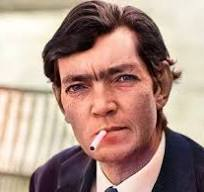
\includegraphics[width=0.5\textwidth]{imagen_cortazar}
\end{frame}
	
		%pdfplumber.open() = se utiliza para ir a la dirección del pdf, retornando una instancia de la% clase $pdfplumber.PDF$ 
%$pdf.pages[]$ = es una propiedad de la clase $pdfplumber.PDF$, la cual se puede indexar para acceder a %las paginas del pdf representadas en la clase $pdfplumber.Page$
%$.extract_text()$ = Método de la clase $pdfplumber.Page$, recopila todos los objetos de caracteres de %la página en un sol string.
%$split('\_n')$ = Divide el string que se genero antes en los saltos de pagina, generando una lista de %lineas.
%$re.findall()$ =
%$.endswith()$ =
%$.strip()$ =
%$.isdigit()$ =
\begin{frame}{Idea general}
	El objetivo es mejorar la representación del corpus uniendo palabras que aparecen juntas con alta frecuencia en el mismo contexto.
	\begin{itemize}
		\item Buscar palabras frecuentes.
		\item Analizar sus contextos más comunes.
		\item Unirlas si aparecen juntas frecuentemente.
	\end{itemize}
\end{frame}

% ==========================================
\begin{frame}[fragile]{Funciones principales}
	\begin{lstlisting}[language=Python]
def palabras_frecuentes_en_contexto(corpus, palabra_objetivo, contexto=1):
	frecuencias = {}
	for i in range(len(corpus)):
		if corpus[i] == palabra_objetivo:
			for j in range(i - contexto, i + contexto + 1):
				if j != i and 0 <= j < len(corpus):
					palabra_contexto = corpus[j]
					frecuencias[palabra_contexto] = frecuencias.get(palabra_contexto, 0) + 1
	return sorted(frecuencias.items(), key=lambda x: x[1], reverse=True)
	\end{lstlisting}
\end{frame}

% ==========================================
\begin{frame}[fragile]{Visualización del contexto}
	\begin{center}
		\begin{tikzpicture}[scale=1, every node/.style={font=\small}]
			\node[draw, fill=blue!10, rounded corners] (a1) at (0,0) {el};
			\node[draw, fill=blue!10, rounded corners] (a2) at (1.5,0) {gato};
			\node[draw, fill=red!10, rounded corners] (a3) at (3,0) {negro};
			\node[draw, fill=blue!10, rounded corners] (a4) at (4.5,0) {dormía};
			\node[draw, fill=blue!10, rounded corners] (a5) at (6,0) {tranquilo};
			
			\draw[thick, red, ->] (a3) -- (a2) node[midway, above] {-1};
			\draw[thick, red, ->] (a3) -- (a4) node[midway, above] {+1};
			
			\node[below=0.4cm of a3] {Contexto = 1 alrededor de negro};
		\end{tikzpicture}
	\end{center}
\end{frame}

% ==========================================
\begin{frame}[fragile]{Unir palabras frecuentes en contexto}
	\begin{lstlisting}[language=Python]
def unir_palabras_en_contexto(corpus, palabra1, palabra2):
	nuevo_corpus = []
	i = 0
	while i < len(corpus):
		if corpus[i] == palabra1 and i + 1 < len(corpus) and corpus[i + 1] == palabra2:
			nuevo_corpus.append(f"{palabra1} {palabra2}")
			i += 2
		else:
			nuevo_corpus.append(corpus[i])
			i += 1
	return nuevo_corpus
	\end{lstlisting}
\end{frame}

% ==========================================
\begin{frame}{Ejemplo visual de unión}
	\begin{center}
		\begin{itemize}
			\item  Si ambas palabras aparecen frecuentemente juntas y una de ellas suele ser predicha mal muchas veces se hace lo siguiente, por ejemplo: Si el \textbf{token} 'el' es frecuentemente mal predicho, entonces se une a una palabra que frecuenta mucho como 'gato'. No necesariamente se hace de derecha a izquierda.
		\end{itemize}
		\vspace{0.1cm}
		\begin{tikzpicture}[node distance=1cm and 0.6cm, every node/.style={font=\small}]
			\node[draw, fill=blue!10, rounded corners] (a1) {el};
			\node[draw, fill=blue!10, rounded corners, right=of a1] (a2) {gato};
			\node[draw, fill=blue!10, rounded corners, right=of a2] (a3) {negro};
			\node[right=of a3] (dots) {...};
			
			\draw[->, thick, red] (a1.south) .. controls +(down:0.6cm) and +(down:0.6cm) .. (a2.south)
			node[midway, below] {\textbf{Se combinan}};
			
			\node[below=1.3cm of a2, draw, fill=green!10, rounded corners] (new) {el gato};
			\node[right=of new] (rest) {negro ...};
			
		\end{tikzpicture}
	\end{center}
\end{frame}

% ==========================================
\begin{frame}[fragile]{Bucle principal de optimización}
	\begin{lstlisting}[language=Python]
def optimizar_corpus(words, min_frecuencia=200, contexto=1, top_contextos=3, iteraciones=3, frecuencia_min=100):
	corpus_modificado = words.copy()
	for iteracion in range(iteraciones):
		cuenta = contar_palabras(corpus_modificado)
		palabras_objetivo = cuenta[cuenta > min_frecuencia].index
			for palabra_objetivo in palabras_objetivo:
			resultados = palabras_frecuentes_en_contexto(corpus_modificado, palabra_objetivo, contexto)
			
	\end{lstlisting}
\end{frame}


\begin{frame}[fragile]{Bucle principal de optimización}
	\begin{lstlisting}[language=Python]
for palabra_contexto, frecuencia in resultados[:top_contextos]:
	if frecuencia > frecuencia_min:
		corpus_modificado = unir_palabras_en_contexto(
		corpus_modificado, palabra_objetivo, palabra_contexto)
return corpus_modificado
	\end{lstlisting}
\end{frame}
% ==========================================

\begin{frame}{Caso 1: Palabra no suficientemente frecuente}
	\begin{center}
		\begin{itemize}
			\item La palabra no alcanza la frecuencia mínima \texttt{min\_frecuencia} para ser considerada.
			\item No se analizan sus contextos, ni se combinan tokens.
		\end{itemize}
		\vspace{0.2cm}
		
		\begin{tikzpicture}[node distance=1cm and 0.6cm, every node/.style={font=\small}]
			\node[draw, fill=gray!15, rounded corners] (a1) {cucharón};
			\node[draw, fill=blue!10, rounded corners, right=of a1] (a2) {de};
			\node[draw, fill=blue!10, rounded corners, right=of a2] (a3) {sopa};
			\node[right=of a3] (dots) {...};
			
			\node[below=1cm of a2, text=red] (msg) {No se combina: frecuencia insuficiente};
		\end{tikzpicture}
	\end{center}
\end{frame}


\begin{frame}{Caso 2: Palabra entra al bucle, pero sus contextos no califican}
	\begin{center}
		\begin{itemize}
			\item La palabra tiene frecuencia suficiente para entrar al análisis.
			\item Sin embargo, las palabras de su contexto no superan \texttt{frecuencia\_min}, por lo que no se unen.
		\end{itemize}
		\vspace{0.2cm}
		
		\begin{tikzpicture}[node distance=1cm and 0.6cm, every node/.style={font=\small}]
			\node[draw, fill=yellow!10, rounded corners] (a1) {grande};
			\node[draw, fill=blue!10, rounded corners, right=of a1] (a2) {el};
			\node[draw, fill=blue!10, rounded corners, right=of a2] (a3) {cielo};
			\node[right=of a3] (dots) {...};
			
			\draw[->, thick, gray!60, dashed] (a2.south) .. controls +(down:0.6cm) and +(down:0.6cm) .. (a3.south)
			node[midway, below, gray] {no supera umbral};
			
			\node[below=1.2cm of a2, text=gray] (msg) {No se unen pese a aparecer juntas};
		\end{tikzpicture}
	\end{center}
\end{frame}


\begin{frame}{Caso 3: Palabras frecuentes se combinan}
	\begin{center}
		\begin{itemize}
			\item Ambas palabras son frecuentes y aparecen juntas.
			\item Se cumple el umbral de contexto, por lo que se unen.
		\end{itemize}
		\vspace{0.1cm}
		
		\begin{tikzpicture}[node distance=1cm and 0.6cm, every node/.style={font=\small}]
			\node[draw, fill=blue!10, rounded corners] (a1) {el};
			\node[draw, fill=blue!10, rounded corners, right=of a1] (a2) {gato};
			\node[draw, fill=blue!10, rounded corners, right=of a2] (a3) {negro};
			\node[right=of a3] (dots) {...};
			
			\draw[->, thick, red] (a1.south) .. controls +(down:0.6cm) and +(down:0.6cm) .. (a2.south)
			node[midway, below] {\textbf{Se combinan}};
			
			\node[below=1.3cm of a2, draw, fill=green!10, rounded corners] (new) {el gato};
			\node[right=of new] (rest) {negro ...};
		\end{tikzpicture}
	\end{center}
\end{frame}


\begin{frame}{Caso 4: Uniones sucesivas en cadena}
	\begin{center}
		\begin{itemize}
			\item Varias palabras frecuentes cumplen las condiciones y se van uniendo sucesivamente.
			\item Se produce un efecto en cadena en el corpus optimizado.
		\end{itemize}
		\vspace{0.1cm}
		
		\begin{tikzpicture}[node distance=1cm and 0.6cm, every node/.style={font=\small}]
			\node[draw, fill=blue!10, rounded corners] (a1) {el};
			\node[draw, fill=blue!10, rounded corners, right=of a1] (a2) {gato};
			\node[draw, fill=blue!10, rounded corners, right=of a2] (a3) {negro};
			\node[draw, fill=blue!10, rounded corners, right=of a3] (a4) {dormido};
			\node[right=of a4] (dots) {...};
			
			\draw[->, thick, red] (a1.south) .. controls +(down:0.5cm) and +(down:0.5cm) .. (a2.south);
			\draw[->, thick, red] (a2.south) .. controls +(down:0.7cm) and +(down:0.7cm) .. (a3.south);
			\draw[->, thick, red] (a3.south) .. controls +(down:0.9cm) and +(down:0.9cm) .. (a4.south);
			
			\node[below=1.6cm of a3, draw, fill=green!10, rounded corners] (new) {el gato negro dormido};
			\node[right=of new] (rest) {...};
			
		\end{tikzpicture}
	\end{center}
\end{frame}



\section{Fragmentación sin BPE}

\begin{frame}{}
	\centering
	\Large Fragmentación\\
	\vspace{0.8cm}
	\begin{figure}
		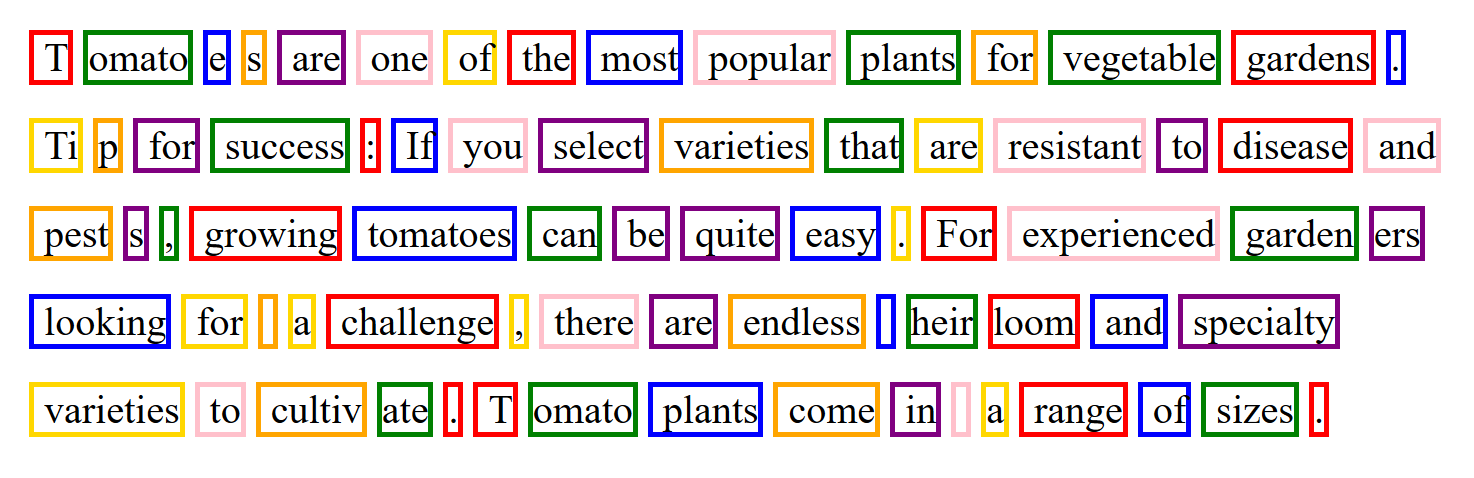
\includegraphics[width=0.5\textwidth]{fm-tokenization}
		\vspace{0.8cm}
		\caption{Imagen extraída de IBM watsonx}
	\end{figure}
\end{frame}

% ======================================================
% 1️⃣ No hay coincidencias en el vocabulario
% ======================================================
\begin{frame}{Caso 1: Ningún token coincide con el vocabulario}
	\begin{center}
		\begin{itemize}
			\item Se recorren las palabras del texto pero ningun token está en el vocabulario.
			\item La función devuelve \texttt{None} tras imprimir el aviso.
		\end{itemize}
		\vspace{0.2cm}
		
		\begin{tikzpicture}[node distance=0.8cm and 0.6cm, every node/.style={font=\small}]
			\node[draw, fill=blue!10, rounded corners] (a1) {brillan};
			\node[draw, fill=blue!10, rounded corners, right=of a1] (a2) {las};
			\node[draw, fill=blue!10, rounded corners, right=of a2] (a3) {estrelinas};
			\node[right=of a3] (dots) {...};
			
			\draw[->, thick, red, dashed] (a3.south) -- ++(0,-0.8)
			node[midway, right, red] {no está en vocab};
			
			\node[below=1.2cm of a2, text=red] (msg) {Retorna None — palabra fuera del vocabulario};
		\end{tikzpicture}
	\end{center}
\end{frame}

% ======================================================
% 2️⃣ Coincidencias parciales (no máximas)
% ======================================================
\begin{frame}{Caso 2: Coincidencias parciales pero no completas}
	\begin{center}
		\begin{itemize}
			\item Se encuentra una parte del texto en el vocabulario, pero no el token más largo posible.
			\item El bucle continúa buscando sin romper correctamente en la posición óptima.
		\end{itemize}
		\vspace{0.2cm}
		
		\begin{tikzpicture}[node distance=0.9cm and 0.6cm, every node/.style={font=\small}]
			\node[draw, fill=blue!10, rounded corners] (a1) {en};
			\node[draw, fill=blue!10, rounded corners, right=of a1] (a2) {la};
			\node[draw, fill=blue!10, rounded corners, right=of a2] (a3) {noche};
			\node[right=of a3] (dots) {...};
			
			\draw[->, thick, orange] (a1.south) .. controls +(down:0.4cm) and +(down:0.4cm) .. (a2.south)
			node[midway, below, orange] {coincide “en”};
			
			\draw[->, thick, gray!60, dashed] (a2.south) .. controls +(down:0.8cm) and +(down:0.8cm) .. (a3.south)
			node[midway, below, gray] {“la noche” no completa};
			
			\node[below=1.4cm of a2, text=orange!90!black] (msg) {Solo se fragmenta lo que se encuentra};
		\end{tikzpicture}
	\end{center}
\end{frame}

% ======================================================
% 3️⃣ Coincidencia exacta (tokenización correcta)
% ======================================================
\begin{frame}{Caso 3: Tokenización exacta con vocabulario}
	\begin{center}
		\begin{itemize}
			\item Se encuentra una secuencia exacta en el vocabulario.
			\item El token se agrega a la lista de salida correctamente.
		\end{itemize}
		\vspace{0.2cm}
		
		\begin{tikzpicture}[node distance=0.9cm and 0.6cm, every node/.style={font=\small}]
			\node[draw, fill=blue!10, rounded corners] (a1) {el};
			\node[draw, fill=blue!10, rounded corners, right=of a1] (a2) {gato};
			\node[draw, fill=blue!10, rounded corners, right=of a2] (a3) {negro};
			
			\draw[->, thick, green!60!black] (a1.south) .. controls +(down:0.5cm) and +(down:0.5cm) .. (a2.south)
			node[midway, below, green!60!black] {coincide “el gato”};
			
			\node[below=1.4cm of a2, draw, fill=green!10, rounded corners] (new) {el gato};
			\node[right=of new] (rest) {negro};
			
			\node[below=0.3cm of new, text=green!50!black] (msg) {Token válido agregado};
		\end{tikzpicture}
	\end{center}
\end{frame}

% ======================================================
% 4️⃣ Coincidencias largas en cascada (subpalabras unidas)
% ======================================================
\begin{frame}{Caso 4: Coincidencias largas y fragmentación en secuencia}
	\begin{center}
		\begin{itemize}
			\item Se van encontrando coincidencias de mayor cantidad de tokens unidos (priorizando tokens más largas).
			\item Se produce una fragmentación por grupos que maximiza coincidencias.
		\end{itemize}
		\vspace{0.1cm}
		
		\begin{tikzpicture}[node distance=0.9cm and 0.6cm, every node/.style={font=\small}]
			\node[draw, fill=blue!10, rounded corners] (a1) {me};
			\node[draw, fill=blue!10, rounded corners, right=of a1] (a2) {gusta};
			\node[draw, fill=blue!10, rounded corners, right=of a2] (a3) {el};
			\node[draw, fill=blue!10, rounded corners, right=of a3] (a4) {helado};
			
			\draw[->, thick, green!60!black] (a1.south) .. controls +(down:0.5cm) and +(down:0.5cm) .. (a2.south);
			\draw[->, thick, green!60!black] (a3.south) .. controls +(down:0.8cm) and +(down:0.8cm) .. (a4.south);
			
			\node[below=1.6cm of a2, draw, fill=green!10, rounded corners] (new1) {me gusta};
			\node[right=of new1, draw, fill=green!10, rounded corners] (new2) {el helado};
			
			\node[below=0.3cm of new1, text=green!50!black] (msg) {Tokenización óptima por grupos};
		\end{tikzpicture}
	\end{center}
\end{frame}


\begin{frame}[fragile]{Fragmentación}
	\begin{lstlisting}[language=Python]
def tokenizar_por_vocab(texto, vocab, indices = False):
	palabras = texto.lower()
	palabras = re.findall(r'\w+|[^\w\s]', palabras, flags=re.UNICODE)
	tokens = []
	i = 0
	n = len(palabras)

	while i < n:
		cand_final = None
		for j in range(n, i, -1):
			cand = " ".join(palabras[i:j])
			if cand in vocab:
				cand_final = cand
				i = j  
				break


	\end{lstlisting}
\end{frame}


\begin{frame}[fragile]{Fragmentación}
	\begin{lstlisting}[language=Python]

if not cand_final:
	cand_final = palabras[i]
	if cand_final not in vocab:
		print(f'palabra: [{cand_final}] no esta en voabulario') 
		return None
i += 1

if indices is False:
	tokens.append(cand_final)
else:
	tokens.append(palabras_a_indice[cand_final])
return tokens
	\end{lstlisting}
\end{frame}


\section{Predicción Consola}

\begin{frame}{}
	\centering
	\Large Generación de texto\\
	\vspace{0.8cm}
	\begin{figure}
		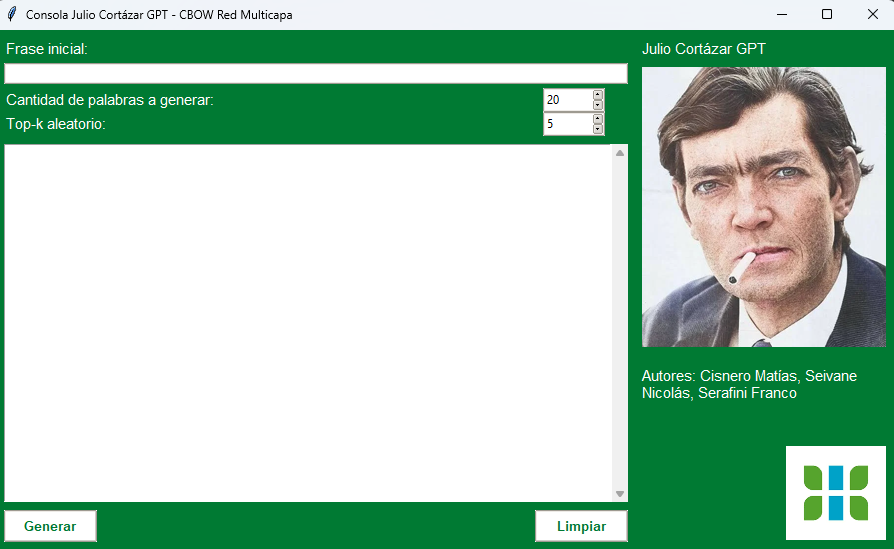
\includegraphics[width=0.5\textwidth]{consola_cortazar_gpt}
		\vspace{0.8cm}
	\end{figure}
\end{frame}
% ======================================================
% CBOW One-Hot — 1️⃣ Construcción de la ventana
% ======================================================
\begin{frame}{CBOW (One-Hot): Construcción de la ventana de contexto}
	\begin{center}
		\begin{itemize}
			\item Las últimas 10 palabras del texto se convierten en índices de vocabulario.
			\item Si hay menos de 10, se repite la última palabra para completar la ventana.
		\end{itemize}
		\vspace{0.2cm}
		
		\begin{tikzpicture}[node distance=0.8cm and 0.4cm, every node/.style={font=\small}]
			\node[draw, fill=blue!10, rounded corners] (a1) {el};
			\node[draw, fill=blue!10, rounded corners, right=of a1] (a2) {gato};
			\node[draw, fill=blue!10, rounded corners, right=of a2] (a3) {negro};
			\node[draw, fill=blue!10, rounded corners, right=of a3] (a4) {duerme};
			\node[right=of a4] (dots) {...};
			
			\draw[decorate, decoration={brace, amplitude=5pt}, thick] (a1.north west) -- (a4.north east)
			node[midway, above=5pt] {Ventana de contexto};
			
			\node[below=1cm of a2, draw, fill=orange!10, rounded corners] (vec) {Índices → Embedding};
			\node[below=0.3cm of vec, text=orange!80!black] (msg) {Cada palabra → vector de embedding};
		\end{tikzpicture}
	\end{center}
\end{frame}


% ======================================================
% CBOW One-Hot — 2️⃣ Predicción de probabilidad
% ======================================================
\begin{frame}{CBOW (One-Hot): Predicción de palabra siguiente}
	\begin{center}
		\begin{itemize}
			\item El modelo predice un vector de embedding para la palabra objetivo.
			\item Devuelve una distribución de probabilidad (\texttt{softmax}), del tamaño one-hot del vocabulario.
			\item Se elige aleatoriamente una palabra del top-\(k\).
		\end{itemize}
		\vspace{0.4cm}
		
		\begin{tikzpicture}[node distance=1cm and 0.6cm, every node/.style={font=\small}]
			\node[draw, fill=orange!10, rounded corners] (x) {Ventana One-Hot};
			\node[draw, fill=yellow!15, rounded corners, right=of x] (m) {Modelo CBOW};
			\node[draw, fill=green!10, rounded corners, right=of m] (out) {Distribución Softmax};
			
			\draw[->, thick] (x) -- (m);
			\draw[->, thick] (m) -- (out);
			
			\node[below=0.8cm of out, text=green!60!black] (msg) {Se elige la palabra más probable (o aleatoria del top-k)};
		\end{tikzpicture}
	\end{center}
\end{frame}


% ======================================================
% CBOW Embedding — 1️⃣ Construcción de ventana con embeddings
% ======================================================
\begin{frame}{CBOW (Embeddings): Construcción de la ventana}
	\begin{center}
		\begin{itemize}
			\item Como en el caso anterior, se concatenan los \textbf{embeddings} de cada palabra.
			\item Si hay menos de 10 palabras, se repite la última embedding.
		\end{itemize}
		\vspace{0.2cm}
		
		\begin{tikzpicture}[node distance=1cm and 0.4cm, every node/.style={font=\small}]
			\node[draw, fill=blue!10, rounded corners] (a1) {el};
			\node[draw, fill=blue!10, rounded corners, right=of a1] (a2) {gato};
			\node[draw, fill=blue!10, rounded corners, right=of a2] (a3) {negro};
			\node[right=of a3] (dots) {...};
			
			\draw[->, thick, orange] (a1.south) -- ++(0,-0.8) node[midway, left] {embedding};
			\draw[->, thick, orange] (a2.south) -- ++(0,-0.8);
			\draw[->, thick, orange] (a3.south) -- ++(0,-0.8);
			
			\node[below=1cm of a2, draw, fill=orange!10, rounded corners] (embs) {Embeddings concatenados};
		\end{tikzpicture}
	\end{center}
\end{frame}


% ======================================================
% CBOW Embedding — 2️⃣ Predicción en espacio vectorial
% ======================================================
\begin{frame}{CBOW (Embeddings): Predicción y similitud}
	\begin{center}
		\begin{itemize}
			\item El modelo predice un vector de embedding para la palabra objetivo.
			\item Se calcula la similitud coseno con todos los embeddings del vocabulario.
			\item Se elige la palabra más similar (o una del top-\(k\)).
		\end{itemize}
		\vspace{0.1cm}
		
		\begin{tikzpicture}[node distance=1cm and 0.6cm, every node/.style={font=\small}]
			\node[draw, fill=orange!10, rounded corners] (x) {Ventana Embeddings};
			\node[draw, fill=yellow!15, rounded corners, right=of x] (m) {Modelo};
			\node[draw, fill=green!10, rounded corners, right=of m] (out) {Embedding predicho};
			
			\draw[->, thick] (x) -- (m);
			\draw[->, thick] (m) -- (out);
			
			\node[below=1.2cm of out, draw, fill=blue!10, rounded corners] (sim) {Similitud coseno con vocabulario};
			\draw[->, thick, green!60!black] (out.south) -- (sim.north);
			
			\node[below=0.3cm of sim, text=green!60!black] (msg) {Se elige la palabra más similar};
		\end{tikzpicture}
	\end{center}
\end{frame}


\begin{frame}[fragile]{Predicción One-hot}
	\begin{lstlisting}[language=Python]
def predecir_cbow_onehot(palabras, modelo, indice_a_palabras, indices_a_embeddings, palabras_a_indice, topk=5):

	palabras_a_indice = globals().get('palabras_a_indice')
	
	tokens_idx = tokenizar_por_vocab(palabras, palabras_a_indice, indices=True)
	
	if tokens_idx is None or len(tokens_idx) == 0:
	return None
	
	if len(tokens_idx) < 10:
		tokens_idx = tokens_idx + [tokens_idx[-1]] * (10 - len(tokens_idx))
	else:
		tokens_idx = tokens_idx[-10:]
	

	\end{lstlisting}
\end{frame}

\begin{frame}[fragile]{Predicción One-hot}
	\begin{lstlisting}[language=Python]
ventana = np.concatenate([indices_a_embeddings[idx] for idx in tokens_idx]).flatten()
pred = modelo.predict(ventana.reshape(1, -1), verbose=0)
probs = np.asarray(pred).flatten()

candidatos = np.argsort(-probs)
topk_indices = candidatos[:topk]
top1 = np.random.choice(topk_indices)
palabra = indice_a_palabras[top1]
return palabra
	\end{lstlisting}
\end{frame}

\begin{frame}[fragile]{Predicción Representación Contextual}
	\begin{lstlisting}[language=Python]
ventana = np.concatenate([W[idx] for idx in tokens_idx]).flatten()
pred_emb = modelo.predict(ventana.reshape(1, -1), verbose=0)
pred_emb = np.asarray(pred_emb).flatten()

sims = cosine_similarity(pred_emb.reshape(1, -1), W)[0]

topk_idx = np.argsort(-sims)[:topk]

top1 = np.random.choice(topk_idx)
palabra_predicha = indice_a_palabras[top1]

return palabra_predicha
	\end{lstlisting}
\end{frame}

\begin{frame}{Estructura Multicapa}
	\begin{center}
		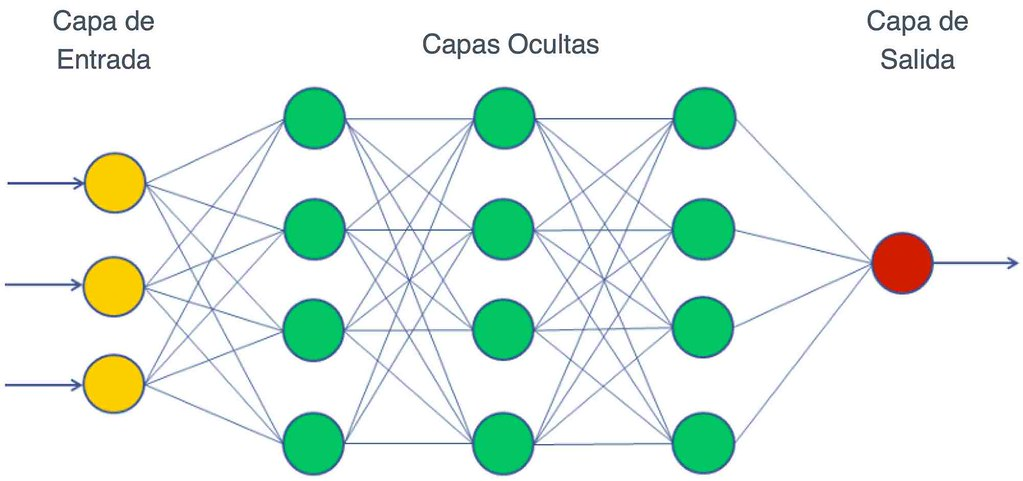
\includegraphics[width=0.7\textwidth]{redes perceptron multicapa.jpg}
		
		\vspace{0.5em}
		{\tiny Créditos: Antonio Richaud}
	\end{center}
\end{frame}


	
\begin{frame}{Estructura Multicapa}
	\small
	\textbf{Modelo:} se implementó una red neuronal de tipo \textbf{Perceptrón Multicapa (PMC)} utilizando la librería \textbf{Keras} (TensorFlow).\\[0.4em]
	
	\textbf{Entradas:} vector resultante de concatenar los embeddings de una \textbf{ventana de 8 palabras previas}, donde cada palabra está representada por su embedding individual.\\[0.4em]

	\textbf{Salida:} vector correspondiente a la palabra objetivo del contexto.\\[0.4em]
	
	\textbf{Arquitectura:}
	\begin{itemize}
		\item Capa oculta 1: 512 neuronas, activación \texttt{gelu}.
		\item Capa oculta 2: 256 neuronas, activación \texttt{gelu}.
		\item Capa oculta 3: 128 neuronas, activación \texttt{gelu}.
		\item Capa de salida: $N$ neuronas, activación \texttt{sigmoid}.
	\end{itemize}
	
	\textbf{Optimizador:} \texttt{Adam} con \texttt{learning rate = 0.0001}.\\
	\textbf{Función de pérdida:} \texttt{MSE (error cuadrático medio)}.
\end{frame}

%-----------------------------------------------------------
\begin{frame}{Entrenamiento del Modelo}
	\small
	El modelo fue entrenado con el corpus embebido, aplicando la función sigmoide a los datos para su normalización.\\[0.5em]
	
	\textbf{Parámetros principales:}
	\begin{itemize}
		\item Épocas: 250
		\item Ventana de contexto: 8 palabras
		\item Error mínimo alcanzado: \textbf{0.0794}
	\end{itemize}
	
	
\end{frame}

\begin{frame}[fragile]{Generación de Texto}
	\small
	La generación de texto se realiza a partir de una secuencia inicial de palabras.
	
	\vspace{0.5em}
	\textbf{Código:}
	\begin{verbatim}
		poner codigo
	\end{verbatim}
	
	\vspace{0.5em}
	La función realiza:
	\begin{enumerate}
		\item Lectura de la secuencia inicial.
		\item Predicción de la siguiente palabra según el tipo de salida.
		\item Evita repeticiones consecutivas de palabras.
		\item Actualiza la ventana de contexto y repite hasta completar la longitud deseada.
	\end{enumerate}
\end{frame}


%-----------------------------------------------------------
\begin{frame}{Resultados de la Predicción}
	\small
	Dado un conjunto de 8 palabras previas, el modelo entrenado con Keras fue capaz de generar una secuencia de palabras consecutivas dentro del corpus.\\[0.5em]
	
	\textbf{Entrada inicial:}
	\begin{quote}
		\textit{``hola como esta usted la noche de hoy''}
	\end{quote}
	
	\textbf{Texto generado:}
	\begin{quote}
		\textit{``diarios mirará saliéramos encegueció creas autopista . admirativamente , saliéramos encegueció feudal creas saliéramos admirativamente encegueció bebida saliéramos contaba encegueció creas saliéramos honorable encegueció creas saliéramos honorable encegueció creas saliéramos''}
	\end{quote}
\end{frame}	

	


	
	
\end{document}